\newpage
\chapter{Ecuación Lineal de Orden Superior}
Antes de introducir el concepto de ecuación lineal de orden superior, primero es necesario generalizar una definición que hicimos al inicio de este documento:
\begin{definicion}[Ecuación Diferencial de orden $m$ y solución]
    Una ecuación diferencial de orden $m\geq 1$ viene dada por una función
    \Func{\Phi}{D\subset\mathbb{R}^{m+2}}{\mathbb{R}}{(t,x_0,x_1,\ldots,x_m)}{\Phi(t,x_0,x_1,\ldots,x_m)}
    continua donde $D$ es un abierto conexo de $\mathbb{R}^{m+2}$.\newline
    Una solución de dicha ecuación diferencial será una función $x:I\rightarrow\mathbb{R}$ con $I\subseteq \mathbb{R}$ intervalo abierto tal que:
    \begin{enumerate}[label=(\roman*)]
        \item $x$ es $m$ veces derivable en $I$.
        \item $(t,x(t),x'(t),x''(t), \ldots, x^{(m)}(t))\in D$ $\forall t\in I$.
        \item $\Phi(t,x(t),x'(t),x''(t),\ldots,x^{(m)}(t)) = 0$ $\forall t\in I$.
    \end{enumerate}
\end{definicion}~\\

\noindent
En esta sección, estaremos interesados en resolver ecuaciones lineales de orden superior. Es decir, las que son de la forma:
\begin{equation}\label{eq:linealsup}
    x^{(m)} + a_{m-1}(t) x^{(m-1)} + \cdots + a_1(t) x' + a_0(t)x = b(t) \qquad m\geq 1
\end{equation}
con $a_0,a_1,\ldots, a_{m-1},b:I\rightarrow\mathbb{R}$ funciones continuas definidas en un intervalo abierto.\\

\noindent
En dicho caso, estaremos ante una ecuación lineal de orden $m$.

\begin{definicion}
    Una ecuación diferencial lineal se dice: 
    \begin{itemize}
        \item homogénea si $b(t) = 0$ $\forall t\in I$.
        \item completa si $b(t) \neq 0$ para algún $t\in I$.
    \end{itemize}
\end{definicion}

\begin{ejemplo}
    Mostramos a continuación varios ejemplos de ecuaciones lineales que motivarán su estudio durante este Capítulo.
    \begin{enumerate}
        \item El caso $m=1$ ha sido ya estudiado anteriormente, se trata de la ecuación lineal de primer orden:
            \begin{equation*}
                x' + a_0(t)x = b(t)
            \end{equation*}
            Por tanto, esta sección estará dedicada a las ecuaciones lineales de orden 2 o mayor. Recordamos que las ecuaciones diferenciales de orden 2 tienen una gran importancia en la física, gracias a la famosa fórmula de $F=m\cdot a$.
        \item La ecuación del oscilador armónico es una ecuación que representa la posición $x$ de un cuerpo atado a una pared con un muelle a lo largo del tiempo $t$, tal y como mostramos en la Figura~\ref{fig:muelle}:
            \begin{equation*}
                m\ddot{x} + kx = 0
            \end{equation*}

            donde $m$ es la masa del cuerpo y $k$ es la constante de elasticidad del muelle, de forma que si el muelle es muy duro $k$ será muy grande y si es muy blando, $k$ tendrá un valor pequeño.

            \begin{figure}[H]
                \centering
             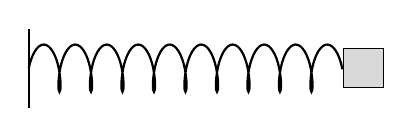
\begin{tikzpicture}
                % Dibuja la pared
                \draw[thick] (0,0.5) -- (0,1.5);

                % Dibuja el muelle
                \draw[thick, decoration={aspect=0.3, segment length=4mm, amplitude=3mm, coil}, decorate] (0,1) -- (4,1);

                % Dibuja el corcho como un cuadrado
                \draw[fill=gray!30] (4,0.75) rectangle (4.5,1.25);
            \end{tikzpicture}               
            \caption{Muelle atado a la pared.}
            \label{fig:muelle}
            \end{figure}

            De esta forma, si estiramos el muelle hacia la derecha, aparecerá una fuerza en sentido contrario. Análogamente, si comprimimos el muelle hacia la izquierda, volverá a aparecer una fuerza en sentido contrario. Se dice que la fuerza de un muelle es una fuerza recuperadora.\\

            La fórmula se deduce a partir de la Segunda Ley de Newton ($F=m\cdot a$) y de la Ley de Hooke, que nos indica que la fuerza de un muelle para una posición del cuerpo $x$ es directamente proporcional a dicha posición:
            \begin{equation*}
                F(x) = -kx
            \end{equation*}
            De esta forma:
            \begin{equation*}
                \left.\begin{array}{rl}
                    F = m\cdot a = m\cdot \ddot{x} \\
                    F(x) = -kx
            \end{array}\right\} \Longrightarrow m\ddot{x} = -kx \Longleftrightarrow m\ddot{x} + kx = 0
            \end{equation*}
            Que es una ecuación diferencial lineal de orden 2, ya que como $m\neq 0$, podemos dividir la expresión entre $m$, obteniendo que:
            \begin{equation*}
                \ddot{x} + \dfrac{k}{m}x = 0
            \end{equation*}
            Por lo que trabajamos con las funciones $a_0,a_1,b:\mathbb{R}\rightarrow\mathbb{R}$ dadas por:
            \begin{equation*}
                a_0(t) = \dfrac{k}{m} \qquad a_1(t) = 0 \qquad b(t) = 0 \qquad t\in \mathbb{R}
            \end{equation*}
        \item Como un último ejemplo de ecuación lineal que se maneja en la práctica y que es de un orden mayor que 2, en ingeniería se trabaja mucho con la ecuación que describe las vibraciones de un puente a lo largo del tiempo, que resulta en una ecuación de cuarto grado.
    \end{enumerate}
\end{ejemplo}~\\

Una vez motivado el uso e importancia de las ecuaciones lineales de orden superior, pasamos a desarrollar la teoría matemática que sustenta este tipo de ecuaciones, la cual está basada en un resultado que enunciaremos pero que se demostrará en el siguiente Capítulo (por no disponer de las herramientas necesarias por ahora).\\

Este resultado es un teorema que nos da la existencia y unicidad de una solución para cada tipo de ecuación lineal de orden $m$ (siendo $m$ cualquier número natural mayor o igual que 1), una vez fijada una condición inicial que esta función solución ha de cumplir.

\begin{definicion}[Condición inicial]
    Dada una ecuación diferencial lineal de orden $m$ cuyos coeficientes están definidos en un intervalo $I$, dar una condición inicial para dicha ecuación será dar un punto $t_0\in I$ y $m$ valores $\alpha_0,\alpha_1,\ldots,\alpha_{m-1}\in \mathbb{R}$ de forma que exijamos que para que una función $x:J\rightarrow\mathbb{R}$ (con $J\subseteq I$) sea solución de dicha ecuación, entonces ha de cumplir la condición inicial, es decir, ha de cumplir que:
    \begin{equation*}
        x(t_0) = \alpha_0, \qquad x'(t_0) = \alpha_1,\qquad  \ldots, \qquad  x^{(m-1)}(t_0) = \alpha_{m-1}
    \end{equation*}
    a parte de ser solución de dicha ecuación diferencial.
\end{definicion}~\\

De esta forma, para dar una condición inicial sobre una ecuación lineal de orden $m$, habrá que exigir $m$ ``condiciones'' sobre un mismo punto $t_0\in I$, que serán el valor de la función y de sus sucesivas derivadas (hasta la $(m-1)$-ésima) en dicho punto.

\begin{ejemplo}
    Para la ecuación del oscilador armónico:
    \begin{equation*}
        x'' + \dfrac{k}{m}x = 0
    \end{equation*}

    \begin{enumerate}
        \item Una condición inicial es exigir, por ejemplo:
            \begin{equation*}
                x(t_0) = 0 \qquad x'(t_0) = 1
            \end{equation*}

            En dicho caso, la condición inicial tiene sentido físico, ya que estaremos diciendo que en el instante $t_0$, que entendemos como el origen temporal del movimiento:
            \begin{itemize}
                \item El muelle parte del origen (posición 0) o posición de equilibrio.
                \item El muelle comienza con velocidad 1 (por lo que le hemos dado un impulso al muelle).
            \end{itemize}
            De forma intuitiva, vemos que una vez dadas una posición y velocidad iniciales al muelle, somos capaces de recrear todo el movimiento que este realizará (de forma sencilla, sabemos que el muelle se estirará y que su elasticidad ejercerá una fuerza en sentido contrario), con lo que seremos capaces de describir su posición $x$ a lo largo del tiempo $t$, con lo que para dicha condición inicial, se espera un único movimiento del muelle (una única solución de la ecuación diferencial).\\

        \item Por otra parte, la condición
            \begin{equation*}
                x(t_0) = 1 \qquad x'(t_0) = 0
            \end{equation*}
            Establece que:
            \begin{itemize}
                \item El muelle parte en la posición inicial resultado de desplazar el cuerpo conectado al muelle una unidad a la derecha (según la Figura~\ref{fig:muelle}) de la posición de equilibrio, con lo que el muelle comienza estirado.
                \item El muelle no tiene velocidad inicial.
            \end{itemize}
            En este caso, podemos pensar que una vez comience a pasar el tiempo (se vaya aumentando $t$ de forma progresiva), veremos que se ejercerá una fuerza hacia la izquierda del cuerpo, como resultado de haber estirado el muelle en un inicio, con lo que también seremos capaces de describir un único movimiento para dicho muelle en estas condiciones iniciales.
    \end{enumerate}
\end{ejemplo}

Este ejemplo nos ha servido para darnos cuenta de que, una vez fijada una condición inicial sobre un movimiento (sobre una ecuación diferencial), seremos capaces de describir la posición del móvil gracias a ese movimiento y dichas condiciones iniciales de forma única.

Por tanto, podemos ya sospechar que dar una condición inicial sobre una ecuación lineal de cualqueir orden $m$ nos es suficiente para encontrar una única solución de dicha ecuación, intuición que se manifiesta a través del siguiente teorema.

\begin{teo}[Existencia y unicidad de las soluciones]\label{teo:existencia_unicidad}
    Dada una ecuación lineal de orden $m$ cuyos coeficientes están definidos en un intervalo $I$ y dados $t_0\in I$, $\alpha_0,\alpha_1,\ldots,\alpha_{m-1}\in \mathbb{R}$ que conforman una condición inicial para dicha ecuación.

    Entonces, existe una única solución $x$ de dicha ecuación diferencial, definida en todo el intervalo $I$, que cumple las condiciones iniciales, es decir:
    \begin{equation*}
        x(t_0) = \alpha_0, \qquad x'(t_0) = \alpha_1,\qquad  \ldots, \qquad  x^{(m-1)}(t_0) = \alpha_{m-1}
    \end{equation*}

    % // TODO: Poner esto al final de la asignatura
    % \begin{proof}
        % La demostración se encuentra en el Teorema~\ref{HACER REFERENCIA}, para el cual será necesario primero repasar algunos conceptos.
    % \end{proof}
\end{teo}

Notemos que, a parte de que el teorema nos da la existencia y unicidad de las soluciones para cualquier ecuación lineal de orden $m$ (que no es poco), además nos garantiza que siempre que dicha ecuación lineal esté definida en un dominio $D=I\times J$, las soluciones estarán siempre definidas en todo el intervalo $I$, algo que no sucede con las ecuaciones diferenciales que no son lineales.

\begin{ejemplo}
    La ecuación diferencial con condición inicial:
    \begin{equation*}
        x' = x^2 \qquad x(0) = 1
    \end{equation*}

    se encuentra definida en el dominio $D=\mathbb{R}^2$, siendo sus soluciones
    \begin{equation*}
        x(t) = \dfrac{1}{1-t} \qquad t\in \left]-\infty,1\right[
    \end{equation*}

    Que no están definidas en todo $\mathbb{R}$.
\end{ejemplo}

Una vez observada la importancia de que las soluciones están definidas en todo el intervalo $I$, notemos que el Teorema~\ref{teo:existencia_unicidad} nos asegura que podemos usar las condiciones iniciales para ``etiquetar'' las soluciones de la ecuación diferencial, tal y como hacíamos en el ejemplo del muelle.\\

\begin{observacion}
    Cuando definimos una ecuación diferencial lineal de orden $m$ no tuvimos en cuenta un detalle de la definición, el cual mostraremos ahora, una vez visto el Teorema~\ref{teo:existencia_unicidad}, y es que en la definición de una ecuación lineal de orden $m$, no consideramos un coeficiente $a_m(t)$ como sí hacemos con el resto de coeficientes, sino que sólamente consideramos el caso $a_m(t) = 1$ $\forall t\in I$.\\

    Notemos que si tenemos una ecuación de la forma:
    \begin{equation*}
        a_m(t)x^{(m)} + a_{m-1}(t) x^{(m-1)} + \cdots + a_1(t)x' + a_0(t)x = b(t)
    \end{equation*}
    en la que $a_m(t) \neq 0$ $\forall t\in I$ (que para nosotros no es lineal de orden $m$), entonces podemos dividir la ecuación entera entre $a_m(t)$, obteniendo una ecuación diferencial lineal de orden $m$ con coeficientes distintos (todos ellos divididos entre $a_m$).\\

    Por tanto, este tipo de ecuaciones diferenciales no serán problema para nosotros, pero sí lo serán aquellas en las que $\exists t\in I$ tal que $a_m(t) = 0$, ya que dichas ecuaciones diferenciales no serán para nosotros ecuaciones lineales. Esto se debe a que para este tipo de ecuaciones, el Teorema~(\ref{teo:existencia_unicidad}) no es cierto, tal y como mostramos en el siguiente ejemplo.
\end{observacion}

\begin{ejemplo}
    Consideremos la ecuación diferencial
    \begin{equation*}
        tx'-x = 0
    \end{equation*}
    con dominio $D=\mathbb{R}^2$, que tiene como familia de funciones solución las rectas que pasan por el origen, tal y como vemos en la Figura~\ref{fig:familia_rectas_origen}:
    \begin{equation*}
        x(t) = ct \qquad c\in \mathbb{R}, \quad t\in \mathbb{R}
    \end{equation*}

\begin{figure}[H]
\centering    
\begin{tikzpicture}
    % Ejes coordenados
    \draw[-Stealth] (-3,0) -- (3,0) node[right] {$t$};
    \draw[-Stealth] (0,-2) -- (0,2) node[above] {$x$};

    % Dibujar las rectas para diferentes valores de c
    \draw[thick, gray!80]   (-3, -2) -- (3, 2);   % c = 1
    \draw[thick, gray!80]  (-3, -2) -- (3, 2);   % c = 0.5
    \draw[thick, gray!80] (-3, -1) -- (3, 1);   % c = 0.25
    \draw[thick, gray!80](-3, 2) -- (3, -2);   % c = -1
    \draw[thick, gray!80](-3, 2) -- (3, -2);   % c = -0.5
    \draw[thick, gray!80] (-3, 1) -- (3, -1);   % c = -0.25
\end{tikzpicture}
\caption{Familia de rectas que pasan por el origen.}
\label{fig:familia_rectas_origen}
\end{figure}
    Sin embargo, esta ecuación diferencial no es una ecuación lineal de orden 1, ya que tenemos como coeficientes $a_0,a_1,b:\mathbb{R}\rightarrow\mathbb{R}$ dados por
    \begin{equation*}
        a_0(t) = -1 \qquad a_1(t) = t \qquad b(t) = 0 \qquad t\in \mathbb{R}
    \end{equation*}
    y tenemos que $a_1(0) = 0$.\\

    Como hemos dicho anteriormente, no consideramos a este tipo de ecuaciones diferenciales como ecuaciones diferenciales lineales, y lo hacemos por una razón justificada, y es que para este tipo de ecuaciones podemos encontrar condiciones iniciales que no nos den una única solución, de forma que a veces tengamos varias soluciones para una misma condición inicial, así como que en otros casos directamente no existe una solución:

    \begin{enumerate}
        \item Si consideramos como condición inicial $x(0) = 0$, entonces tendremos infinitas soluciones de la ecuación diferencial, ya que todas las rectas de la familia anterior pasan por el punto $(0,0)$, con lo que todas ellas cumplen la ecuación inicial y son solución de la ecuación diferencial, no se cumple la unicidad.
        \item Si ahora consideramos como condición inicial $x(0)=1$, entonces no tenemos ninguna solución para la ecuación diferencial que cumpla esta condición inicial, ya que la recta vertical que pasa por el origen no forma parte de dicha familia de soluciones de la ecuación, por no ser una función. No se cumple la existencia.
    \end{enumerate}
    Por tanto, la definición de ecuación diferencial lineal va asociada al Teorema~\ref{teo:existencia_unicidad}, con lo que es otro indicador de su importancia.\\

    Sin embargo, si queremos trabajar ante este tipo de ecuaciones, como en este caso $a_1$ solo se anula en un punto, podemos considerar la ecuación lineal de orden 1:
    \begin{equation*}
        x' - \dfrac{x}{t} = 0
    \end{equation*}
    definida bien en $D^+ = \mathbb{R}^+\times \mathbb{R}$, bien en $D^- = \mathbb{R}^-\times \mathbb{R}$ y en cada caso obtenemos una ecuación lineal.

    A pesar de ello, lo que estamos haciendo es quedarnos con parte de las soluciones anteriores de forma que se cumpla la existencia y unicidad, al eliminar toda la recta $t=0$ del problema.
\end{ejemplo}~\\

Ya hemos comentado anteriormente que la demostración del Teorema~\ref{teo:existencia_unicidad} la dejamos para el siguiente Capítulo por no estar preparados para realizarla. Sin embargo, podemos ya demostrar un resultado más débil, que nos enuncia el teorema para el caso $m=1$:

\begin{prop}[Existencia y unicidad para ecuaciones lineales de orden 1]
    \ \\
    Dada una ecuación lineal de orden 1:
    \begin{equation*}
        x' + a_0(t)x = b(t)
    \end{equation*}
    con $a_0,b:I\rightarrow\mathbb{R}$ funciones continuas en un intervalo $I$ y dados $t_0\in I$, $\alpha_0\in \mathbb{R}$.

    Entonces, existe una única solución $x$ de la ecución lineal, definida en todo el intervalo $I$ que cumple la condición inicial, es decir:
    \begin{equation*}
        x(t_0) = \alpha_0 
    \end{equation*}
    
    \begin{proof}
        Necesitamos pues, demostrar la existencia y unicidad de dicha solución $x$:
        \begin{description}
            \item [Existencia.]~\\
                Veamos que el problema de valores iniciales
                \begin{equation*}
                    x' + a_0(t)x = b(t) \qquad x(t_0) = \alpha_0
                \end{equation*}
                tiene una solución $x$ que cumple las propiedades enuncidas. Sea pues $x:I\rightarrow\mathbb{R}$ una función dada por:
                \begin{equation*}
                    x(t) = e^{-A_0(t)} [\alpha_0 + F(t)] \qquad t\in I
                \end{equation*}

                donde $A_0,F:I\rightarrow\mathbb{R}$ son funciones definidas por
                \begin{equation*}
                    A_0(t) = \int_{t_0}^{t} a_0(s)~ds \qquad F(t) = \int_{t_0}^{t} e^{A_0(s)}b(s)~ds  \qquad t\in I
                \end{equation*}

                las cuales están bien definidas gracias al Teorema Fundamental del Cálculo, por ser $a_0$ y $e^{A_0}b$ funciones continuas en $I$ (la segunda por ser producto de una función continua por una composición de funciones continuas), con lo que $x$ está bien definida.

                Además, el Teorema Fundamental del Cálculo nos garantiza que $A_0,F\in C^1(I)$, con lo que $x\in C^1(I)$. Veamos que $x$ cumple la condición inicial y que es solución de la ecuación lineal de orden 1:

                \begin{itemize}
                    \item Por una parte, calculamos el valor de $x(t_0)$, teniendo en cuenta que:
                        \begin{align*}
                            A_0(t_0) &= \int_{t_0}^{t_0} a_0(s)~ds  = 0 \\
                            F(t_0) &= \int_{t_0}^{t_0} e^{A_0(s)}b(s)~ds = 0
                        \end{align*}

                        con lo que:
                        \begin{equation*}
                            x(t_0) = e^{-A_0(t_0)}(\alpha_0 + F(t_0)) = e^0 (\alpha_0 + 0) = \alpha_0
                        \end{equation*}
                    \item Por otra, parte, derivamos $x$ para comprobar si cumple con la ecuación diferencial, usando para ello la derivada del producto:
                        \begin{equation*}
                            x'(t) = -a_0(t)e^{-A_0(t)} [\alpha_0 + F(t)] + e^{-A_0(t)}e^{A_0(t)}b(t) \AstIg -a_0(t) x(t) + b(t)
                        \end{equation*}
                        Donde en $(\ast)$ hemos aplicado que:
                        \begin{equation*}
                            x(t) = e^{-A_0(t)} [\alpha_0 + F(t)]
                        \end{equation*}
                \end{itemize}
                Notemos que para que $x$ fuera solución era suficiente con coger como $A_0$ cualquier primitiva de $a_0$ y como $F$ cualquier primitiva de $e^{A_0}b$. Sin embargo, para que $x$ cumpliera la condición inicial, hemos tomado aquellas integrales indefinidas centradas en $t_0$.

            \item [Unicidad.]~\\
                Supongamos que tenemos dos soluciones de la ecuación lineal de orden 1 $x_1,x_2:I\rightarrow\mathbb{R}$ que cumplen con la condición inicial, es decir:
                \begin{equation*}
                    x_1(t_0) = \alpha_0 = x_2(t_0)
                \end{equation*}
                y tratamos de demostrar que dichas funciones son iguales. Para ello, definidmos $y:I\rightarrow\mathbb{R}$ dada por:
                \begin{equation*}
                    y(t) = x_1(t) - x_2(t) \qquad t\in I
                \end{equation*}

                Como $x_1,x_2$ son soluciones de la ecuación diferencial lineal, entonces son de clase $C^1(I)$, con lo que $y\in C^1(I)$ y podemos calcular su derivada:
                \begin{align*}
                    y'(t) &= x_1'(t) - x_2'(t) = -a_0(t)x_1(t) + \cancel{b(t)} + a_0(t)x_2(t) - \cancel{b(t)} \\
                          &= -a_0(t) (x_1(t) - x_2(t)) = -a_0(t)y(t) \qquad \forall t\in I
                \end{align*}
                De esta forma, si $x_1$ y $x_2$ eran soluciones de la ecuación lineal completa, resulta que $y$ es solución de la ecuación lineal homogénea asociada a dicha ecuación.\\

                Además, resulta que $y$ cumple con la condición inicial $y(t_0) = 0$:
                \begin{equation*}
                    y(t_0) = x_1(t_0) - x_2(t_0) = \alpha_0 - \alpha_0 = 0
                \end{equation*}
                Con vistas a demostrar que $y$ es constantemente igual a 0, lo que haremos será resolver la ecuación diferencial 
                \begin{equation*}
                    y' + a_0(t) y = 0
                \end{equation*}

                buscando un factor integrante para dicha ecuación. En el capítulo anterior, vimos que el factor integantes para esta ecuación era $\mu(t,x) = e^{A_0(t)}$, con lo que multiplicamos la ecuación diferencial, obteniendo que:
                \begin{equation*}
                    e^{A_0(t)}y'(t) + a_0(t)e^{A_0(t)}y(t) = 0
                \end{equation*}

                con lo que estamos ante una ecuación exacta, de forma que podemos pensar dicha expresión como la derivada de una función de una variable:
                \begin{equation*}
                    \dfrac{d}{dt}\left(e^{A_0(t)}y(t)\right) = 0
                \end{equation*}
                Como consecuencia, tenemos que las soluciones de la ecuación diferencial son de la forma:
                \begin{equation*}
                    e^{A_0(t)} y(t) = c \qquad c\in \mathbb{R} \quad t\in I
                \end{equation*}
                Sin embargo, como no buscamos todas las soluciones, sólo buscamos aquella que cumple que $y(t_0) = 0$, llegamos a que $c = 0$, con lo que la expresión de la función $y$ es:
                \begin{equation*}
                    y(t) = 0 \qquad \forall t\in I
                \end{equation*}
                Concluimos que $x_1(t) = x_2(t)$ $\forall t\in I$.
        \end{description}
    \end{proof}
\end{prop}

La demostración para el caso $m=1$ no es difícil, por lo que nos preguntamos qué es lo que hace que al pasar a cualquier $m$ esta se complique.

Resulta que a partir de las ecuaciones lineales de orden 2 no podemos encontrar una fórmula que nos describa las soluciones de la ecuación lineal. De hecho, puede demostrarse que la ecuación de Riccati (estudiada anteriormente) no tiene fórmula, así como que cualquier ecuación lineal de segundo orden puede pasarse a una ecuación de Riccati, por lo que es imposible encontrar una fórmula para una función $x$ solución de una ecuación lineal de orden 2.\\

% // TODO: Clase 18 Nov

Veamos esto (que la ecuación lineal de orden mayor o igual que 2 no tiene fórmula):
Sea una ecuación lineal homogénea de segundo orden:
\begin{equation*}
    x'' + a_1(t) x' + a_0(t) x = 0
\end{equation*}
Resulta que hay una relación entre esta ecuación y la de Riccati de 1er orden:

Supongamos que $x:J\rightarrow\mathbb{R}$ es una solución de dicha ecuación definida en un intervalo $J\subseteq I$ en donde $x(t) \neq 0$ $\forall t\in J$. ($x\in C^2(J)$).

Definimos $y:J\rightarrow\mathbb{R}$ dada por:
\begin{equation*}
    y(t) = \dfrac{x'(t)}{x(t)}
\end{equation*}
Que es de clase $C^1(J)$, por ser $x'\in C^1(J)$ y $x(t) \neq 0$ $\forall t\in J$. Derivando:
\begin{equation*}
    y' = \dfrac{x'' x - {(x')}^{2}}{x^2}
\end{equation*}
Ahora, utilizamos que $x$ es solución de la ecuación lineal de segundo orden homogénea:
\begin{equation*}
    y' = \dfrac{x'' x - {(x')}^{2}}{x^2} = \dfrac{(-a_1x' - a_0 x)x {(x')}^{2}}{x^2} \AstIg -a_1 y - a_0 -y^2
\end{equation*}
Donde en $(\ast)$ usamos que $y = \frac{x'}{x}$. Con lo que $y$ es una función que cumple:
\begin{equation*}
    y' = -a_1(t)y - a_0(t) - y^2
\end{equation*}
Que es una ecuación de Riccati.

Esta es la relación que hay entre una ecuación lineal homogénea de segundo orden y una ecuación de Riccati de primer orden.


Por tanto, como Riccati no se puede resolver en general (no tiene fórmula), concluimos que la ecuación lineal homogenea de segundo grado no se puede resolver en general.

No hay esperanza de encontrar una fórmula general.\\


Si ahora tenemos una ecuación de segundo orden, si conocemos una solución distinta de la trivial (homogénea), podemos hayar todas sus soluciones.
La de 3er orden pasa a una de 2o, \ldots.

El camino ha de ser mucho más teórico.
Sin embargo, si los coeficientes son constantes, sí que tenemos fórmula para las ecuaciones lineales.


\section{Espacio vectorial de las funciones}

% // TODO: Definicion de e.v. ?
% Respecto a la suma es un grupo y propiedades con escalares

En esta sección, fijaremos un intervalo (abierto?) $I$ fijo.

\begin{definicion}
    Dado un intervalo $I\subseteq \mathbb{R}$, definimos el conjunto:
    \begin{equation*}
        \bb{F}(I,\mathbb{R}) = \{f:I\rightarrow\mathbb{R} \mid f \text{\ es una aplicación}\}
    \end{equation*}
\end{definicion}

Definimos:
\begin{equation*}
    \bb{F} = \bb{F}(I, \mathbb{R}) = \{f:I\rightarrow\mathbb{R}\}
\end{equation*}
con lo que $f\in \bb{F}$ es una función $f:I\rightarrow\mathbb{R}$. El conjunto de todas las curvas en explícitas.

% // Pasar definiciones a prop. de que con dichas operaciones es un e.v.
\begin{definicion}[Suma de funciones]
    Dadas dos funciones $f,g\in \bb{F}$, definimos la función suma, $f+g:I\rightarrow\mathbb{R}$ dada por:
    \begin{equation*}
        (f+g)(t) = f(t) + g(t) \qquad t\in I
    \end{equation*}
\end{definicion}

% ejemplo de f(t) = t, g(t) = 1-t

\begin{definicion}[]
    \begin{gather*}
        \lm f:I\rightarrow\mathbb{R} \\
        (\lm f)(t) = \lm f(t) \qquad t\in I
    \end{gather*}
\end{definicion}

% ejemplo de f(t) = sent, al multiplicar se multiplica la amplitud de la onda

\begin{prop}
    \begin{itemize}
        \item Las funciones continuas son un subespacio.
        \item Las funciones de clase $k$ son un subespacio.
    \end{itemize}
\end{prop}

\subsubsection{Independencia lineal de funciones}
La independencia vectorial en cada espacio vectorial se manifiesta de una forma distinta.

\begin{definicion}
    En un e.v. $V$, si $v_1,\ldots,v_k \in V$, se dice que son linealmente independientes cuando, dados $\lm_1,\ldots,\lm_k\in \mathbb{R}$, entonces:
    \begin{equation*}
        \lm_1v_1 + \ldots + \lm_k v_k = 0 \Longrightarrow \lm_1 = \cdots = \lm_k = 0
    \end{equation*}
\end{definicion}
Es decir, el vector 0 sólo acepta una única representación como combinacion lineal de dichos vectores.

En nuestro contexto, dadas $f_1,\ldots,f_k\in \bb{F}$, la independecia lineal de esas funciones quiere decir, que, dadas $\lm_1,\ldots,\lm_k\in \mathbb{R}$:
\begin{equation*}
    \lm_1f_1 + \ldots + \lm_k f_k = 0 \Longrightarrow \lm_1 = \cdots = \lm_k = 0
\end{equation*}
es decir:
\begin{equation*}
    \lm_1f_1(t) + \ldots + \lm_k f_k(t) = 0 \qquad \forall t\in I \Longrightarrow \lm_1 = \cdots = \lm_k = 0
\end{equation*}

% // TODO: Definir independencia lineal para cualquier conjunto de vectores
Dado un e.v. $V$ y un conjunto de vectores $S\subseteq V$, entonces $S$ es l.i. si para todo subconjunto finito $F\subseteq S$ y todo conjunto de numeros, la suma es 0 implica 0


La independencia lineal de funciones depende del $I$, de forma que sean indep. en un intervalo mas grande y en un chico sean dependientes, de forma que no sean subespacios.
La independencia lineal va ligada al espacio vectorial.
Diremos que las funciones son linealmente independientes en este intervalo.


% Pasar esto a cualquier espacio $F$
\begin{prop}
    Sea $V\subseteq \bb{F}$ un subespacio vectorial, siendo $f_1,\ldots,f_k\in V$ linealmente independientes $\Longleftrightarrow $ lo son en $\bb{F}$.
\end{prop}


Probar que una serie de funciones son l.i. por derivación:
Dadas $f_1,\ldots,f_k \in \bb{F}$, dados $\lm_1,\ldots,\lm_k\in \mathbb{R}$ tal que:
\begin{equation*}
    \lm_1 f_1(t) + \cdots + \lm_k f_k(t) = 0 \qquad \forall t\in I
\end{equation*}
Suponiendo que $f_i$ son derivables una vez, entonces:
\begin{equation*}
    \lm_1 f_1'(t) + \cdots + \lm_k f_k'(t) = 0 \qquad \forall t\in I
\end{equation*}
Si ahora suponemos que $f_i$ son derivables $h$ veces:
\begin{equation*}
    \lm_1 f_1^{(h)}(t) + \cdots + \lm_k f_k^{(h)}(t) = 0 \qquad \forall t\in I
\end{equation*}
Como tenemos $k$ incógnitas, buscamos $k$ ecuaciones, luego exigimos derivabilidad de $f_i$ $k-1$ veces:
\begin{equation*}
    \left\{\begin{array}{c}
    \lm_1 f_1^{(1)}(t) + \cdots + \lm_k f_k^{(1)}(t) = 0 \qquad \forall t\in I \\
    \lm_1 f_1^{(2)}(t) + \cdots + \lm_k f_k^{(2)}(t) = 0 \qquad \forall t\in I \\
    \vdots \\
    \lm_1 f_1^{(k-1)}(t) + \cdots + \lm_k f_k^{(k-1)}(t) = 0 \qquad \forall t\in I
    \end{array}\right.
\end{equation*}
Entonces, para cada $t\in I$, tenemos una ecuación lineal distinta, donde las incógnitas son los $\lm_i$.

Tenemos $k$ ecuaciones y $k$ incógnitas, luego será sufición necesaria y suficiente para resolverlo que el determinante sea distinto de 0.

En realidad, tenemos (con $A(t)$ una matriz dependiente de $t$):
\begin{equation*}
    A(t) x = 0
\end{equation*}
Donde la solución $x$ no varía, luego nos basta con encontrar la solución para algún $t$.
De esta forma, con que $det(A(t)) \neq 0$ para algún $t$, ya tendremos el sistema resuelto.

\begin{definicion}[Wronskiano]
    Dadas $f_1,\ldots,f_k\in \bb{F}$ funciones derivables $k-1$ veces, definimos su wronskiano como una función $I\rightarrow\mathbb{R}$ dada por:
    \begin{equation*}
        W(f_1,\ldots,f_k)(t) = \left|\begin{array}{ccc}
            f_1(t) & \cdots & f_k(t) \\
            f_1'(t) & \cdots & f_k'(t) \\
            \vdots & \ddots & \vdots \\
            f_1^{(k-1)}(t) & \cdots & f_k^{(k-1)}(t) 
        \end{array}\right| \qquad t\in I
    \end{equation*}
\end{definicion}

\begin{prop}
    Dadas $f_1,\ldots,f_k$ funciones derivables $k-1$ veces en $I$, si existe $t_0\in I$ tal que $W(f_1,\ldots,f_k)(t_0) \neq 0$. Entonces, $f_1,\ldots,f_k$ son linealmente independientes en $I$.
    \begin{proof}
        % // TODO: Hacer
    \end{proof}
\end{prop}

\begin{ejemplo}
    Ejemplos de independencia lineal:
    \begin{itemize}
        \item 
            \begin{equation*}
                W(\sen, \cos)(t) = 1
            \end{equation*}
        \item Consideramos $f_0,f_1,\ldots,f_k:\mathbb{R}\rightarrow\mathbb{R}$ de forma que:
            \begin{equation*}
                f_k(t) = t^k \quad k\geq 1 \qquad f_0(t) = 1 \qquad t\in \mathbb{R}
            \end{equation*}
            Veamos que $f_0,f_1,\ldots,f_k$ son linealmente independientes en $\mathbb{R}$:
            \begin{equation*}
                W(f_0,f_1,\ldots,f_k)(t) = \left|\begin{array}{ccccl}
                    1 & t & t^2 & \cdots & t^k \\
                    0 & 1 & 2t & \cdots & kt^{k-1} \\
                    0 & 0 & 2 & \cdots & k(k-1)t^{k-2} \\
                    \vdots & \vdots & \vdots & \ddots & \vdots \\
                    0 & 0 & 0 & \cdots & k!
                \end{array}\right| = 1\cdot 1\cdot 2\cdot \ldots \cdot k! \neq 0
            \end{equation*}
        \item $f_1(t) = \cos(t^2)$, $f_2(t) = \sen(t^2)$, vamos a probar que son linealmente independientes en $\mathbb{R}$:
            \begin{equation*}
                W(f_1,f_2)(t) = \left|\begin{array}{cc}
                    \cos(t^2) & \sen(t^2) \\
                    -2t\sen(t^2) & 2t\cos(t^2) 
                \end{array}\right| = 2t (\cos^2(t^2) + \sen^2(t^2))= 2t
            \end{equation*}
            Por tanto, el Wronskiano se anula solo en $t=0$.

            \begin{equation*}
                \left.\begin{array}{r}
                    \lm_1 \cos(t^2) + \lm_2\sen(t^2) = 0\\
                    -\lm_1 2t\sen(t^2) + \lm_2 2t\cos(t^2) = 0
                \end{array}\right\}
            \end{equation*}
            tomando $t = \sqrt{\pi}$:
            \begin{equation*}
                \left.\begin{array}{r}
                        -\lm_1 = 0 \\
                        -2\sqrt{\pi} \lm_2 = 0
                \end{array}\right\} \Longrightarrow \lm_1 = \lm_2 = 0
            \end{equation*}
    \end{itemize}
\end{ejemplo}

\begin{ejemplo}
    Ejemplo de Peano para el que el Wronskiano se anula pero no son linalmente independientes:
    \begin{equation*}
        f_1(t) = t^2 \qquad f_2(t) = -|t|t \qquad t\in \mathbb{R}
    \end{equation*}
    Veamos que estas funciones son linealmente independientes en $\mathbb{R}$, pero que el Wronskiano es 0.\\

    Lo que sucede es que a pesar de que las funciones son linealmente independientes, el sistema que generamos nunca es compatible determinado.

    En primer lugar, lo primero es ver que $f_1,f_2$ sean derivables una vez:
    \begin{equation*}
        f_2(t) = -|t|t = \left\{\begin{array}{lr}
                -t^2 & t \geq 0 \\
                t^2 & t<0
        \end{array}\right. \qquad \forall t\in \mathbb{R}
    \end{equation*}
    Con lo que $f_2$ es la unión de dos parábolas, $t^2$ y $-t^2$ unidas por el vértice.
    % // TODO: Graficar f_2

    \begin{equation*}
        f_2'(t) = \left\{\begin{array}{lr}
                -2t & t \geq 0 \\
                2t & t \leq 0
        \end{array}\right. = -2 |t| \qquad \forall t\in \mathbb{R}
    \end{equation*}
    Tenemos que $f_2\in C^1(\mathbb{R})$, pero que $f_2\notin C^2(\mathbb{R})$.

    Aunque la tangente en 0 sea común, se ve que las derivadas segundas no coinciden.

    \begin{equation*}
        W(f_1,f_2)(t) = \left|\begin{array}{cc}
            t^2  & -|t|t \\
            2t & -2|t|
        \end{array}\right| = -2|t|t^2 + 2|t|t^2 = 0 \qquad \forall t\in \mathbb{R}
    \end{equation*}

    % // TODO: Dibujar f_1 junto con f_2
    Se ve a ojo que son linealmente independientes.

    Veamos que $f_1$, $f_2$ son l.i. en $\mathbb{R}$. Por tanto, sean $\lm_1$, $\lm_2 \in \mathbb{R}$.
    \begin{equation*}
        \lm_1 t^2 - \lm_2 |t| t = 0 \qquad \forall t\in \mathbb{R}
    \end{equation*}
    dando valores $t$:
    \begin{equation*}
        \left.\begin{array}{lr}
                t = 1: & \lm_1 - \lm_2 = 0 \\
                t = -1: &\lm_1 + \lm_2 = 0
        \end{array}\right\} \Longrightarrow \lm_1 = \lm_2 = 0
    \end{equation*}
\end{ejemplo}

\subsubsection{Aplicaciones lineales}
Sean $V,W$ espacios vectoriales sobre $\mathbb{R}$, tomamos una aplicación $L:V\rightarrow W$ una aplicación lineal:
\begin{equation*}
    L(v_1 + v_2) = L(v_1) + L(v_2) \qquad L(\lm v) = \lm L(v)
\end{equation*}

\begin{definicion}[Núcleo]
    Dada una aplicación lineal $L:V\rightarrow W$, definimos:
    \begin{equation*}
        \ker L = \{v\in V \mid L(v) = 0\}
    \end{equation*}
\end{definicion}
Abstracción de los sistemas lineales homogéneos.

\begin{prop}
    $\ker L$ es un subespacio vectorial de $V$.
\end{prop}

Cualquier tipo de ecuación que tenga naturaleza lineal puede estudiarse como:
\begin{equation*}
    Lx = b
\end{equation*}
Para cierta matriz $L$ de una aplicación lineal.\\

Hemos de buscar en los espacios y el operador para transformar una ecuación lineal de orden $k$ en dicha expresión.

\begin{equation*}
    Lx = x^{(k)} + a_{k-1}x^{(k-1)} + \ldots + a_1 x' + a_0 x
\end{equation*}
\begin{equation*}
    V = C^k(I) \qquad W = C(I)
\end{equation*}
Es una costumbre escribir:
\begin{equation*}
    L[x] = x^{(k)} + a_{k-1}x^{(k-1)} + \ldots + a_1 x' + a_0 x
\end{equation*}
Y decir que $L$ es una operador (llevar funciones en funciones) diferencial.

De esta forma, podemos ver esta ecuación como:
\begin{equation*}
    L[x] = b
\end{equation*}
Con $b$ una función continua dada por dicha expresión.

\begin{ejemplo}
    Dada la ecuación
    \begin{equation*}
        x'' + t^2 x' - x = b(t)
    \end{equation*}

    con $b:\mathbb{R}\rightarrow\mathbb{R}$ una función continua.\\
    \begin{equation*}
        a_1(t) = t^2 \qquad a_0(t) = -1
    \end{equation*}

    Tenemos un operador $L:C^2(\mathbb{R})\rightarrow C(\mathbb{R})$ tal que:
    \begin{equation*}
        L[x] = x'' + a_1 x' + a_0 x
    \end{equation*}
    y se verifica que $L$ es lineal, por ser la ecuación lineal:
    \begin{equation*}
        L[ax+y] = aL[x] + L[y]
    \end{equation*}

    De esta forma:
    \begin{equation*}
        L[e^t] = e^t + t^2 e^t - e^t = t^2 e^t
    \end{equation*}
\end{ejemplo}

\section{Ecuación lineal homogénea de grado superior}
Dada la ecuación lineal homogénea de orden superior, \ldots
Definimos $L$ como \ldots

Consideramos: 
\begin{equation*}
    Z = \{x \in C^k(I) \mid L[x] = 0\}
\end{equation*}
Este conjunto es el conjunto de soluciones de la ecuación lineal homogénea de orden superior.\\

Notemos que $Z$ es un espacio vectorial:
\begin{equation*}
    Z = \ker L
\end{equation*}

\begin{ejemplo}
    Volviendo al ejemplo de la ecuación diferencial que describe el moviemiento de un muelle:
    \begin{equation*}
        x'' + x = 0
    \end{equation*}
    Soluciones no triviales de la misma son:
    \begin{align*}
        \varphi_1(t) &= \cos t \\
        \varphi_2(t) &= \sen t 
    \end{align*}
    Por tanto, por ser $Z$ un espacio vectorial, todas las combinaciones lineales de $\varphi_1$ y $\varphi_2$ son solución de dicha ecuación:
    \begin{equation*}
        \{c_1\varphi_1 + c_2\varphi_2 \mid c_1,c_2\in \mathbb{R}\} \subseteq Z
    \end{equation*}
    Un argumento a favor de que se da la igualdad es que es una ecuación de segundo orden, la solución depende de dos parámetros y ya tenemos dos parámetros, de forma intuitiva.

% Acos(wt + \phi) = \alpha_1 cos wt + alpha_2 sen wt

    y $\sen$, $\cos$ son l.i. por su Wronskiano igual a 1.
\end{ejemplo}

\begin{teo}
    \begin{equation*}
        \dim Z = k
    \end{equation*}
    \begin{proof}
        Veremos que es isomorfo (aplicacion lineal biyectiva) con un espacio de la misma dimensión:
        \begin{equation*}
            V\cong W \Longrightarrow \dim V = \dim W
        \end{equation*}
        % Comienza
        Fijado $t_0\in I$, consideramos $\Phi_{t_0}:Z\rightarrow \mathbb{R}^k$ dada por:
        \begin{equation*}
            \Phi_{t_0}(x) = \left(\begin{array}{c}
                x(t_0) \\
                x'(t_0) \\
                \vdots \\
                x^{(k-1)}(t_0)
            \end{array}\right) \qquad x\in Z
        \end{equation*}
        Es fácil ver que $\Phi_{t_0}$ es lineal, por la linealidad de la derivada.\\

        \begin{itemize}
            \item $\Phi_{t_0}$ es un monomorfismo por la unicidad del problema de valores iniciales vista en el Teorema~\ref{teo:existencia_unicidad}, con lo que $\dim Z \leq k$.
            \item $\Phi_{t_0}$ es un epimorfismo por la existencia de las soluciones dada por el Teorema~\ref{teo:existencia_unicidad} ante una condición inicial, con lo que $\dim Z \geq k$.
        \end{itemize}
        Concluimos que $\dim Z = k$.
    \end{proof}
\end{teo}


